
%(BEGIN_QUESTION)
% Copyright 2006, Tony R. Kuphaldt, released under the Creative Commons Attribution License (v 1.0)
% This means you may do almost anything with this work of mine, so long as you give me proper credit

Some processes may be controlled by an automatic controller only having {\it integral} control action.  Here is a schematic diagram of one such controller:

$$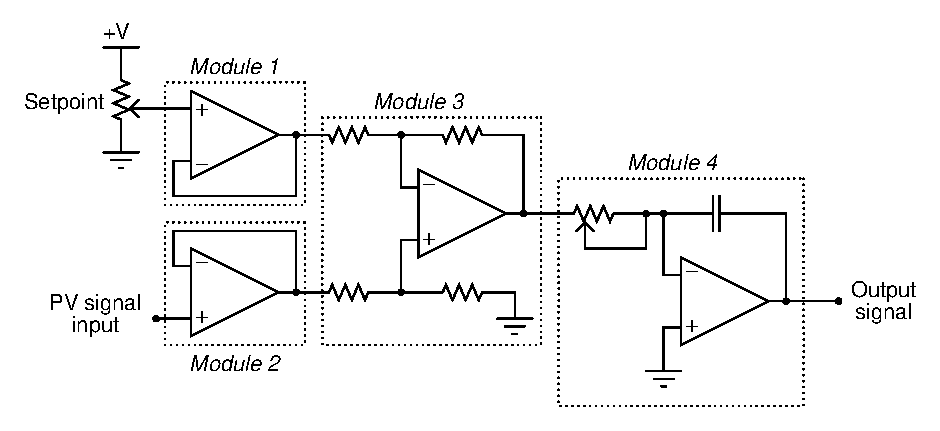
\includegraphics[width=15.5cm]{i01588x01.eps}$$

Examine this schematic diagram and then answer the following questions about it:

\begin{itemize}
\item{} Show where ``error'' is calculated in the circuit
\item{} Determine whether this is a direct-acting controller or a reverse-acting controller
\item{} Identify how to {\it decrease} the integration time constant ($\tau_i$); i.e. how to {\it increase} the aggressiveness of integral action
\end{itemize}

\vskip 20pt \vbox{\hrule \hbox{\strut \vrule{} {\bf Suggestions for Socratic discussion} \vrule} \hrule}

\begin{itemize}
\item{} If used to control a real process, would this controller suffer from {\it offset} like a proportional-only controller would?  Explain why or why not?
\item{} Identify the effects of the feedback wire in module 2 failing open.
\item{} Identify the effects of the lower-left resistor in module 3 failing open.
\item{} Identify the effects of the upper-left resistor in module 3 failing open.
\item{} Identify the effects of the lower-right resistor in module 3 failing open.
\item{} Identify the effects of the upper-right resistor in module 3 failing open.
\item{} Identify the effects of the capacitor in module 4 failing shorted.
\end{itemize}

\underbar{file i01588}
%(END_QUESTION)





%(BEGIN_ANSWER)

\begin{itemize}
\item{} Show where ``error'' is calculated in the circuit: {\bf At the output of the differential amplifier circuit (module 3)}
\item{} Determine whether this is a direct-acting controller or a reverse-acting controller: {\bf Reverse-acting}
\item{} Identify how to {\it decrease} the integration time constant ($\tau_i$); i.e. how to {\it increase} the aggressiveness of integral action: {\bf Smaller capacitor in module 4, lesser potentiometer setting in module 4, increased differential voltage gain in module 3}
\end{itemize}

%(END_ANSWER)





%(BEGIN_NOTES)


%INDEX% Control, integral: analog electronic controller

%(END_NOTES)


